
\documentclass[journal]{IEEEtran}

\hyphenation{op-tical net-works semi-conduc-tor}

\usepackage{dcolumn}
\usepackage{colortbl}
\usepackage{graphicx}
\usepackage{rotating}

\begin{document}
%
% paper title
\title{Proyecto con la Oficina de Responsabilidad Social Universitaria - PUJ, Cali.}
\author{Alejandro~Cardona,~\IEEEmembership{}
        Luis~Santiago~Osorio,~\IEEEmembership{}
        Diego~Lozada,~\IEEEmembership{}% <-this % stops a space
\thanks{}% <-this % stops a space
\thanks{}}

\markboth{}

\maketitle


\IEEEpeerreviewmaketitle
\section{\textbf{Control de Versiones}}

\begin{tabular}{|>{\columncolor[gray]{0.7}} c |c|}
\hline
Vercion &\makebox[6.5cm][c]{2.0}\\
\hline
Fecha & 17/10/2012\\
\hline
\end{tabular}

\begin{tabbing}
\hspace*{2cm} 
\end{tabbing}


En esta version, se cambia el formato de documento para manejar la herramienta {\LaTeX}, para un mejor uso de el formato de la IEEE, y se generan los nuevos cambios en el proyecto con respecto a las reuniones en el periodo actual.

\section{\textbf{Contexto}}
La oficina de responsabilidad social es la encargada del manejo de
proyectos relacionados con Responsabilidad Social de la Pontificia
Universidad Javeriana Cali. Se encarga de analizar el impacto de los
proyectos.

\section{\textbf{Introduccion}}

\subsection{Proposito}
\PARstart{E}{l} siguiente documento especificara las principales caracteristicas del proyecto con la oficina de responsabilidad social, mostrando el contexto, los actores que intervienen, la tecnologia utilizada y los diferentes requerimientos funcionale y no funcionales de la aplicacion.


\subsection{Alcance}
Se obtendr\'a una aplicaci\'on capas de gestionar \'e ingresar,
los proyectos relacionados con responsabilidad social, y mostrar las estad\'isticas que hagan una buena
muestra de los datos que se estraer\'an de la base de datos del sistema.

El sistema quedara dise\~nado en Java y podra realizar los siguentes procesos:

\begin{enumerate}
\item Agregar proyectos
\item Gestionar:
\begin{enumerate}
\item Crear.
\item Aceptar.
\item Clasificar.
\item Modificar.
\end{enumerate}
\item Generar estadisticas.
\item Generar Datos.
\end{enumerate}

\section{\textbf{Descripci\'on general}}

El sistema será un producto diseñado para trabajar en entorno web, lo que permitirá su utilización de forma remota, además trabajará de manera independiente por lo tanto no interactuará con otros sistemas.\\\\
El sistema permitir\'a realizar las siguientes funciones:\\
\begin{itemize}
\item
\textbf{Administraci\'on de proyectos:} El administrador del sistema podr\'a gestionar los proyectos (agregar, modificar, eliminar, buscar, aceptar).
\item
\textbf{Prevalidaci\'on de proyectos:} El sistema hara una prevalidaci\'on de los proyectos recividos y enviara una alerta a el administrador.
\item
\textbf{Generaci\'on de estadisticas:} El sistema podra generar estadisticas a partir de los proyectos almacenados en la base de datos.
\item
\textbf{Envio de Proyectos:} El sistema permitira el envio de proyectos, por parte de el administrador y de usuarios externos previamente registrados.
\item
\textbf{Busqueda de proyectos:} El sistema podra tener campo de busqueda, en el que dependiendo de el actor, generara la busqueda.

\end{itemize}

\section{\textbf{Personal Involucrado}}

\begin{tabular}{|>{\columncolor[gray]{0.7}} c |c|}
\hline
Nombre &\makebox[5cm][c]{ Diego Alexander Lozada}\\
\hline
Rol & Programador\\
\hline
Categor\'ia profesional & Ingeniero de Sistemas y \\
&Computaci\'on\\
\hline
Responsabilidades & Codificar y Documentar\\
&la aplicaci\'on\\
\hline
\end{tabular}

\begin{tabbing}
\hspace*{1cm} 
\end{tabbing}

\begin{tabular}{|>{\columncolor[gray]{0.7}} c |c|}
\hline
Nombre &\makebox[5cm][c]{ Alejandro Cardona}\\
\hline
Rol & Programador\\
\hline
Categor\'ia profesional & Ingeniero de Sistemas y \\
&Computaci\'on\\
\hline
Responsabilidades & Codificar y Documentar \\
&la aplicaci\'on\\
\hline
\end{tabular}

\begin{tabbing}
\hspace*{1cm} 
\end{tabbing}

\begin{tabular}{|>{\columncolor[gray]{0.7}} c |c|}
\hline
Nombre &\makebox[5cm][c]{ Luis Santiago Osorio}\\
\hline
Rol & Programador\\
\hline
Categor\'ia profesional & Ingeniero de Sistemas y \\
&Computaci\'on\\
\hline
Responsabilidades & Codificar y Documentar \\
&la aplicaci\'on\\
\hline
\end{tabular}

\begin{tabbing}
\hspace*{1cm} 
\end{tabbing}

\begin{tabular}{|>{\columncolor[gray]{0.7}} c |c|}
\hline
Nombre &\makebox[4.5cm][c]{ Juan Carlos Mart\'inez}\\
\hline
Rol & Profesor de Ingenier\'ia de spftware\\
\hline
Categor\'ia profesional & Ingeniero de Sistemas y \\
&Computaci\'on\\
\hline
Responsabilidades & Controlar los Avances del proyecto\\
\hline
\end{tabular}

\begin{tabbing}
\hspace*{1cm} 
\end{tabbing}

\begin{tabular}{|>{\columncolor[gray]{0.7}} c |c|}
\hline
Nombre &\makebox[7cm][c]{ Claudia Mora}\\
\hline
Rol & Cliente\\
\hline
\end{tabular}

\begin{tabbing}
\hspace*{1cm} 
\end{tabbing}

\begin{tabular}{|>{\columncolor[gray]{0.7}} c |c|}
\hline
Nombre &\makebox[7cm][c]{ \'Angela Mar\'ia}\\
\hline
Rol & Cliente\\
\hline
\end{tabular}

\begin{tabbing}
\hspace*{1cm} 
\end{tabbing}

\section{\textbf{Tecnologia}}
Info Tecnologia

\section{\textbf{Arquitectura del sistema}}

\begin{center}
\rotatebox{0}{\scalebox{1}[1]{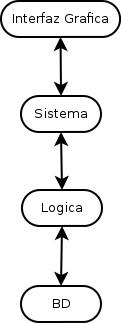
\includegraphics[width=3cm,height=4cm]{Diagrama4.png}}}
\end{center}


\section{\textbf{Requerimientos}}

\begin{enumerate}
\item
En sistema tendra un logeo, para el ingreso de los usuarios, ya sea externos o por parte de la oficina de responsabilidad social(administradores).\\
\item
El sistema, debera permitir el envio de proyectos, por parte de los usuarios y los administradores.\\
\item
El sistema deberá hacer una prevalidaci\'on de los proyectos ingresados
por los usuarios en la p\'agina. En esta pre validaci\'on se tendr\'an en
cuenta el an\'alisis de los datos ingresados en una encuesta indicada, que se genera a partir de los tres tipos de proyectos:
\begin{itemize}
\item
Proyectos por Facultad o internos a la universidad.
\item
Proyectos con Paz y Bien.
\item
Proyectos de la compa\~nia jesuita.\\
\end{itemize}
\item
El sistema podra gestionar los proyectos ingresados a el sistema, dando la posibilidad de agregar,eliminar,modificar los proyectos.\\
\item
El sistema permitira la busqueda de proyectos, por categoria, poblacion o un parametro espesificado por el usuario. En esta busqueda dependiendo del usuario logeado se mostrata informacion mas detallada de los proyecto, es decir, si el usuario es un administrador podra visualisar informacion mas detallada de los proyectos, y si el usuario no lo es, visualizara una vercion muy especifica de los datos.\\
\item
El sistema podra generar estadisticas, a partir de los datos ya almacenados en el sistema. Dichas estadisticas se calcularan, tomando en cuenta los vs mas significativos para la oficina de responsabilidad social.\\ 
\item
El sistema deberá enviar una alerta al administrador, informando de
un nuevo proyecto enviado por el sistema.
\end{enumerate}

\section{\textbf{Especificaci\'on de Requerimientos Funcionales}}
\begin{enumerate}

\item
Requerimiento No 1.
\begin{itemize}
\item
Software: Aplicaci\'on Java
\item
Version: 1.0
\item
Nombre del Requerimiento: Logeo
\item
Descripci\'on: El sistema permitira el logeo de los usuarios para dar privilegios de administrador o de usuario normal.
\item
Involucrados: Usuario
\item
Precondiciones: 
\begin{itemize}
\item
El sistema debe haber iniciado
\end{itemize}
\item
Excepciones: 
\item
Funciones Relacionadas:
\item
Documentos Relacionados:
\item
Realizado por: Luis Osorio, Alejandro Cardona, Diego Lozada.
\item
Fecha: 17/10/2012.
\item
Acciones: 
\end{itemize}
\begin{tabular}{|l|l|}
\hline
\makebox[3.75cm][c]{\textbf{Usuario}} &\makebox[3.75cm][c]{\textbf{Sistema}}\\
\hline
Inicia la aplicacion &\\
\hline
& Muestra la ventana de logeo\\
\hline
Ingresa los datos&\\
\hline
& Verifica\\
\hline
& Muestra ventana de usuario\\
\hline
\end{tabular}
\begin{tabbing}
\hspace*{1cm} 
\end{tabbing}

\item
Requerimiento No 2.
\begin{itemize}
\item
Software: Aplicaci\'on Java.
\item
Version: 1.0.
\item
Nombre del Requerimiento: Envio de Proyecto.
\item
Descripci\'on: El sistema permitira el envio de proyectos al sistema.
\item
Involucrados: Usuario.
\item
Precondiciones:
\begin{itemize}
\item
El usuario debe haberse logeado.
\end{itemize}
\item
Excepciones: 
\item
Funciones Relacionadas: logeo
\item
Documentos Relacionados: PDF o WORD adjunto al proyecto.
\item
Realizado por: Luis Osorio, Alejandro Cardona, Diego Lozada.
\item
Fecha: 17/10/2012
\item
Acciones: 
\end{itemize}
\begin{tabular}{|l|l|}
\hline
\makebox[3.75cm][c]{\textbf{Usuario}} &\makebox[3.75cm][c]{\textbf{Sistema}}\\
\hline
llena el formulario y &\\
adjunta el archivo&\\
\hline
Envia el proyecto& \\
\hline
& Se guarda el proyecto \\
&en la aplicaci\'on\\
\hline
& Envia cponfirmaci\'on de\\
&envio\\
\hline
\end{tabular}
\begin{tabbing}
\hspace*{1cm} 
\end{tabbing}

\item
Requerimiento No 3.
\begin{itemize}
\item
Software: Aplicaci\'on Java
\item
Version: 1.0
\item
Nombre del Requerimiento: Validaci\'on 
\item
Descripci\'on: El sistema validara los proyectos enviados a el sistema, cejecutando la prevalidacion, para continuar el proceso de aprobaci\'on por el administrador o de rechazo, segun el caso.
\item
Involucrados: Usuario, Administrador
\item
Precondiciones: 
\begin{itemize}
\item
El usuario debe haberse logeado.
\end{itemize}
\item
Excepciones: Formato incorrecto.
\item
Funciones Relacionadas: Logeo.
\item
Documentos Relacionados: 
\item
Realizado por: Luis Osorio, Alejandro Cardona, Diego Lozada.
\item
Fecha: 17/10/2012.
\item
Acciones: 
\end{itemize}
\begin{tabular}{|l|l|}
\hline
\makebox[3.75cm][c]{\textbf{Usuario}} &\makebox[3.75cm][c]{\textbf{Sistema}}\\
\hline
Envia Formulario&\\
\hline
& Ejecuta validaci\'on\\
\hline
& Genera reporte\\
\hline
\end{tabular}
\begin{tabbing}
\hspace*{1cm} 
\end{tabbing}

\item
Requerimiento No 4.
\begin{itemize}
\item
Software: Aplicaci\'on Java
\item
Version: 1.0
\item
Nombre del Requerimiento:Gestion de Proyectos. 
\item
Descripci\'on: El sistema otorgara opciones a el administrador para el manejo de los proyectos como eliminaci\'on, aceptaci\'on, modificaci\'on.
\item
Involucrados: Administrador
\item
Precondiciones: 
\begin{itemize}
\item
El usuario debe haberse logeado.
\item
Debe haber proyectos en el sistema
\end{itemize}
\item
Excepciones: 
\item
Funciones Relacionadas: Logeo.
\item
Documentos Relacionados: 
\item
Realizado por: Luis Osorio, Alejandro Cardona, Diego Lozada.
\item
Fecha: 17/10/2012.
\item
Acciones: 
\end{itemize}
\begin{tabular}{|l|l|}
\hline
\makebox[3.75cm][c]{\textbf{Administrador}} &\makebox[3.75cm][c]{\textbf{Sistema}}\\
\hline
Selecciona Proyecto&\\
\hline
& Muestra Opciones de \\
& gestion del proyecto\\
\hline
Selecciona opcion&\\
\hline
&Ejecuta opcion\\
\hline
&Informa si la tarea a sido\\&
 realizada correctamente\\
\hline
\end{tabular}
\begin{tabbing}
\hspace*{1cm} 
\end{tabbing}

\item
Requerimiento No 5.
\begin{itemize}
\item
Software: Aplicaci\'on Java
\item
Version: 1.0
\item
Nombre del Requerimiento:Busqueda de proyectos. 
\item
Descripci\'on: El sistema tendra opci\'on de busqueda, que mostrara los datos buscados dependiendo de el usuario que realize dicha busqueda.
\item
Involucrados: Administrador, Usuario.
\item
Precondiciones:
\begin{itemize}
\item
El usuario debe haberse logeado.
\end{itemize}
\item
Excepciones: Si el usuario no es administrador, visualizara solo los datos basicos de el proyecto buscado.
\item
Funciones Relacionadas: Logeo.
\item
Documentos Relacionados: 
\item
Realizado por: Luis Osorio, Alejandro Cardona, Diego Lozada.
\item
Fecha: 17/10/2012.
\item
Acciones - Administrador: 
\end{itemize}
\begin{tabular}{|l|l|}
\hline
\makebox[3.75cm][c]{\textbf{Administrador}} &\makebox[3.75cm][c]{\textbf{Sistema}}\\
\hline
Busca Proyecto&\\
\hline
& Muestra lista de proyectos\\
& asociada a la busqueda\\
\hline
Selecciona proyecto&\\
\hline
&Muestra informaci\'on\\
\hline
\end{tabular}
\begin{tabbing}
\hspace*{1cm} 
\end{tabbing}

\item
Requerimiento No 6.
\begin{itemize}
\item
Software: Aplicaci\'on Java
\item
Version: 1.0
\item
Nombre del Requerimiento:Generaci\'on de estadisticas. 
\item
Descripci\'on: El sistema generara estadisticas que podra seleccionar de una lista de opciones.
\item
Involucrados: Administrador.
\item
Precondiciones:
\begin{itemize}
\item
El usuario debe haberse logeado.
\end{itemize}
\item
Excepciones: 
\item
Funciones Relacionadas: Logeo.
\item
Documentos Relacionados: 
\item
Realizado por: Luis Osorio, Alejandro Cardona, Diego Lozada.
\item
Fecha: 17/10/2012.
\item
Acciones - Administrador: 
\end{itemize}
\begin{tabular}{|l|l|}
\hline
\makebox[3.75cm][c]{\textbf{Administrador}} &\makebox[3.75cm][c]{\textbf{Sistema}}\\
\hline
Entra en el menu de &\\
estadisticas&\\
\hline
& Muestra opciones de \\
&estadisticas\\
\hline
Selecciona opcion&\\
\hline
&Genera y muestra\\
&la estadistica \\
&seleccionada\\
\hline
\end{tabular}
\begin{tabbing}
\hspace*{1cm} 
\end{tabbing}

\item
Requerimiento No 7.
\begin{itemize}
\item
Software: Aplicaci\'on Java
\item
Version: 1.0
\item
Nombre del Requerimiento:Alerta de proyectos. 
\item
Descripci\'on: El sistema generara una alerta a el administrador, coda ves que un proyecto enviado a el sistema aya pasado la prevalidaci\'on.
\item
Involucrados: Administrador - Usuario.
\item
Precondiciones:
\begin{itemize}
\item
Un proyecto enviado que paso el primer filtro.
\end{itemize}
\item
Excepciones: 
\item
Funciones Relacionadas:
\item
Documentos Relacionados: 
\item
Realizado por: Luis Osorio, Alejandro Cardona, Diego Lozada.
\item
Fecha: 17/10/2012.
\item
Acciones - Administrador: 
\end{itemize}
\begin{tabular}{|l|l|}
\hline
\makebox[3.75cm][c]{\textbf{Usuario}} &\makebox[3.75cm][c]{\textbf{Sistema}}\\
\hline
Envia proyecto&\\
\hline
& Se hace la prevalidaci\'on\\
\hline
& Envia alerta a el\\
& administrador\\

\hline
\end{tabular}
\begin{tabbing}
\hspace*{1cm} 
\end{tabbing}

\end{enumerate}

\section{\textbf{Casos de Uso}}
En esta secci\'on se explicaran, los diferentes ecenarios en los que los usuarios interactuaran con el sistema, y se especificara cada caso de uso usado en el ecenario.\\\\
Actores:
\begin{itemize}
\item  
Administrador.
\item
Usuario Externo.
\end{itemize}

Ecenarios:
\begin{itemize}
\item  
Administrativos.
\item
Busqueda.
\item
Validaciones.\\\\
\end{itemize}

Diagramas de Casos de uso:
\begin{enumerate}
\item 
 Caso de uso numero 1:\\
\begin{center}
\rotatebox{0}{\scalebox{1}[1]{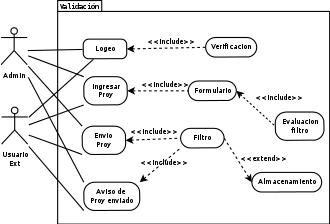
\includegraphics[width=6cm,height=4cm]{Diagrama1.png}}}
\end{center}
\item 
 Caso de uso numero 2:\\
\begin{center}
\rotatebox{0}{\scalebox{1}[1]{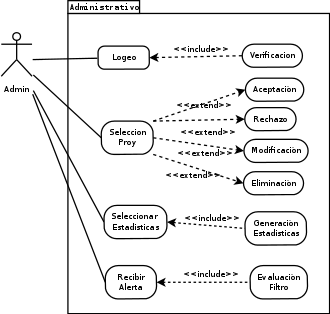
\includegraphics[width=6cm,height=4cm]{Diagrama2.png}}}
\end{center}
\item 
 Caso de uso numero 3:\\
\begin{center}
\rotatebox{0}{\scalebox{1}[1]{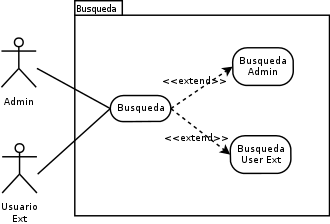
\includegraphics[width=6cm,height=4cm]{Diagrama3.png}}}
\end{center}
\end{enumerate}

\begin{thebibliography}{1}

\bibitem{IEEEhowto:kopka}
H.~Kopka and P.~W. Daly, \emph{A Guide to {\LaTeX}}, 3rd~ed.\hskip 1em plus
  0.5em minus 0.4em\relax Harlow, England: Addison-Wesley, 1999.

\end{thebibliography}
\end{document}


